\chapter{Literature Survey}

\section{The PUF concept}
The simplest sentence to describe PUF is "A PUF is an object's fingerprint" \cite{Reference4}. The fingerprint can represent a specific human in the world, such as the PUF can represent
an object. The fingerprint is inherently created when people was born, and the so does PUF, which is inherently exist in an object according to unique manufacturing random variation \cite{Reference4}.
With the representation and inherent property, the fingerprint and the PUF is said to be unclonable since it is impossible to control and predict human's fingerprint. This is an important concept for PUF. \par

This intrinsic property can be extract from chip which has PUF circuit existed inside \cite{Reference2}. The way PUF works is by entering a certain length of bits(so called challenge) into the PUF, and it will
generate another specific length of bits(so called response). According to the property of PUF that was discuss above, it is impossible to find two different PUF that will produce the same response when entering same challenge(See Figure \ref{fig:figure1}).
\begin{figure}[ht]
\centering
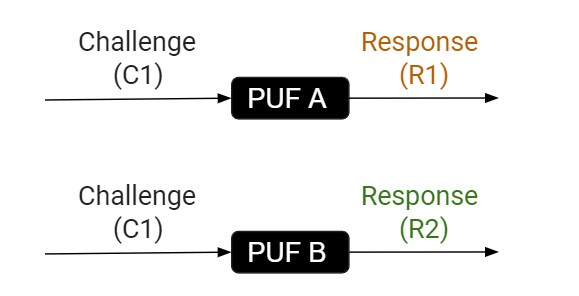
\includegraphics[width=8cm]{figures/figure1.jpg}
\caption{Different PUF that generate different response when input same challenge}
\label{fig:figure1}
\end{figure}

\section{Weak and strong PUF}
PUF can be classified into two categories, weak and strong PUF according to the strength of PUF. The strength of PUF indicate the number of challenge response pairs(so called CRPs) can be generate 
from the PUF \cite{Reference1}. The higher numbers of the CRPs can a PUF generate, the better strength it has. Generally, if increasing the size of the PUF leads to a linear increase in the number of CRPs, it is consider weak PUF. 
On the other hand, if increasing the size of the PUF leads to a exponential increase in the number of CRPs, it is consider strong PUF.\par

For the weak PUF, it represent the PUF that has smaller set of CRPs. While it is impossible to 
create a clone of PUF, but with small set of CRPs, this will allow attacker to record all the CRPs when attacker has physical access to PUF \cite{Reference1}. With the knowledge of CRPs, attacker can easily provide the corresponding
response to challenge as like they have a clone(See Figure \ref{fig:figure2}). The weak PUF can be use for authentication and key storage. However, since weak PUF's CRPs can be fully access, ensure having a secure environment and whether the original PUF is being evaluating is relatively important \cite{Reference1}.
\begin{figure}[ht]
    \centering
    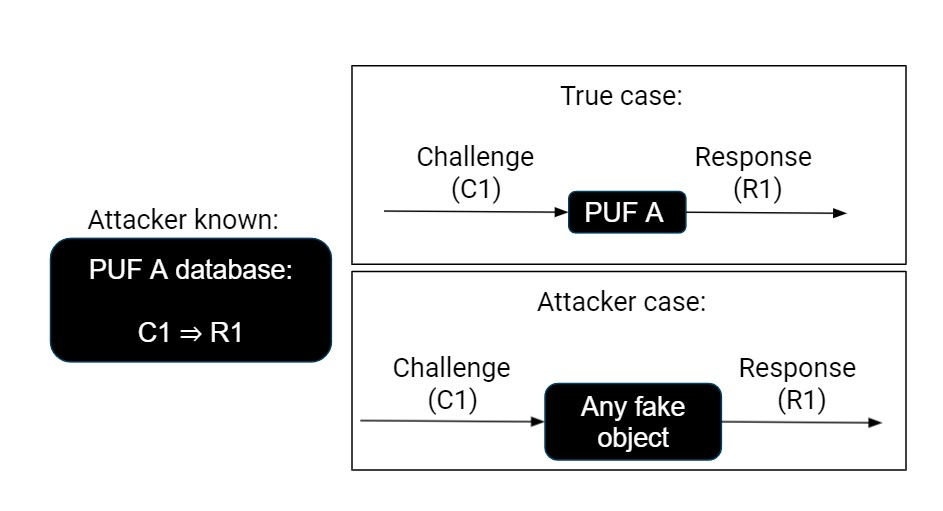
\includegraphics[width=10cm]{figures/figure2.jpg}
    \caption{Attacker can perform same behavior as Weak PUF when have fully access to CRPs and not under secure environment}
    \label{fig:figure2}
    \end{figure}

For strong PUF, means the number of CRPs is significantly large that even attacker get access, having throughout knowledge of CRPs is impossible. While the number of CRPs is so large,
and the CRP are randomly selected in usage, the probability that attacker has knowledge about the CRP currently using is small. In addition, each CRPs that is used once will 
be discarded(See Figure \ref{fig:figure3}) so even if attacker recorded certain CRPs, also called eavesdropped, they will not be able to put them into use. The strong PUF can also be use for authentication but do not need to protect CRPs
as serious as weak PUF.

\begin{figure}[ht]
    \centering
    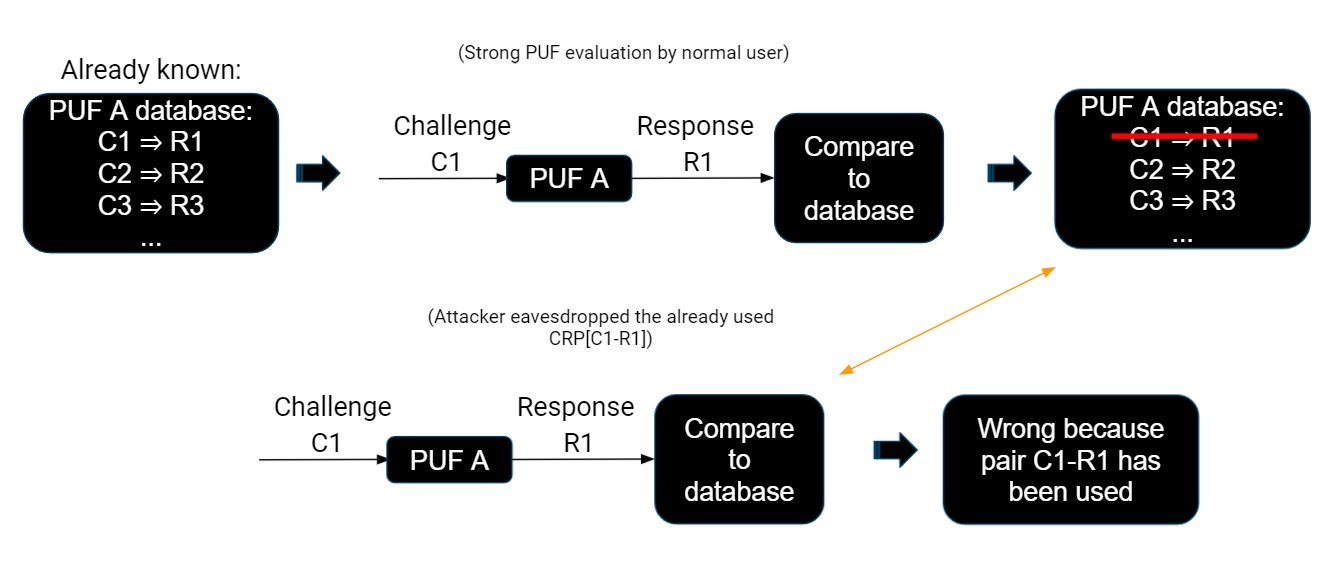
\includegraphics[width=15cm]{figures/figure3.jpg}
    \caption{The attacker eavesdropped CRP that has been used can not successfully validate in next evaluation for strong PUF}
    \label{fig:figure3}
    \end{figure}

\section{Authentication}
One of the application of PUF is authentication. As discuss in Chapter 1's introduction, PUF does not require huge computational power and are cost effective, so it is suitable for many devices,
especially the resources-constraint devices. The PUF's authentication included two stages, enrollment and authentication stage. In the enrollment stage, the company possess the PUF, so
company can connect server to PUF and sent lots of challenges along with recording the CRPs into the database \cite{Reference2} (See Figure \ref{fig:figure4}).

\begin{figure}[ht]
    \centering
    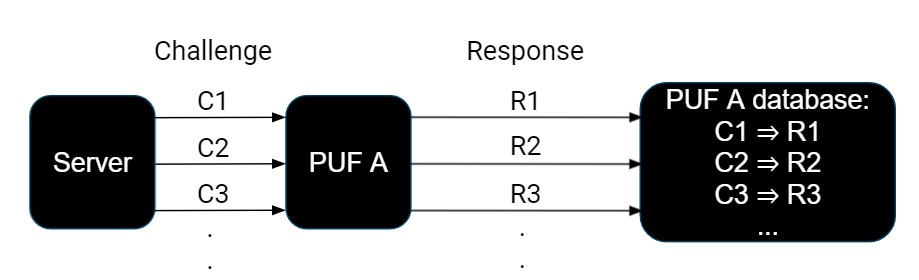
\includegraphics[width=10cm]{figures/figure4.jpg}
    \caption{Enrollment stage in PUF authentication}
    \label{fig:figure4}
    \end{figure}

After recording all the CRPs, the company can now implement PUF on electronic devices.
In the authentication stage, the server sent arbitrary challenge to the devices that contain PUF while the device will return response. Afterward, the server compare the response from the device with the database, 
if the challenge and response pair exist in the database, the device is valid \cite{Reference2} (See Figure \ref{fig:figure5}). A life example will be banking card.

\begin{figure}[ht]
    \centering
    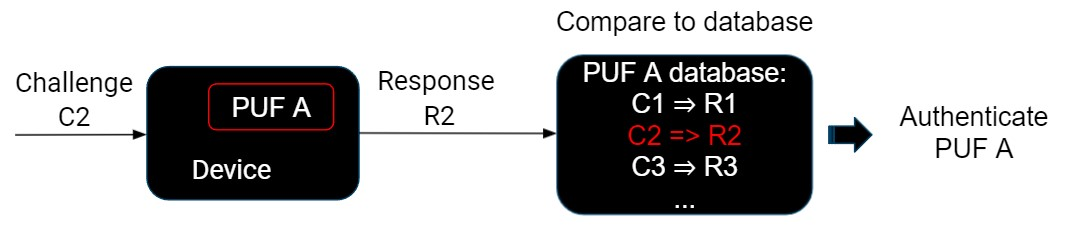
\includegraphics[width=12cm]{figures/figure5.jpg}
    \caption{Authentication stage in PUF authentication}
    \label{fig:figure5}
    \end{figure}

\section{Arbiter PUF and XOR arbiter PUF}
There are many different types of PUF such as arbiter PUF, ring oscillator PUF, lightweight PUF, etc. In this paper, arbiter PUF and its mutation will be introduced in detail. The general idea of
the arbiter PUF is comparing the transition speed for two electrical signal in the PUF's structure(See Figure \ref{fig:figure6}). The arbiter PUF's structure contains a numbers of 
multiplexers and a arbiter, and two multiplexers will combined into a switching box \cite{Reference3}. When enter a challenge bits, bit 1 indicate the upper and lower signal will switch and bit 0 indicate the two signals remain unchanged in each switching box, which will 
eventually form paths for the signals. Then the signals start transferring, the time arrived at the arbiter for two signals is different since each multiplexer and wire has unique delay. The response will be determined by the arbiter. 
The structure is fair, which will not favor one of the path, even there exist bias, a simple solution of adding a delay in the structure can solve the problem. For example, if the arbiter favor the lower path,
by adding a delay to upper path, it can has a head start.
\begin{figure}[ht]
    \centering
    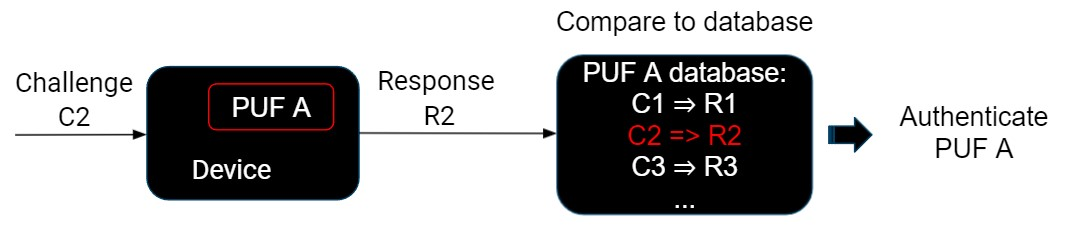
\includegraphics[width=12cm]{figures/figure5.jpg}
    \caption{Arbiter PUF structure}
    \label{fig:figure6}
    \end{figure}

\section{Threat and modeling attack on PUF}


\section{Summary}


